\section{Simplification Queries}
\label{sec:simplification-queries}

In this section, given a fixed polyline, we design a data structure that allows optimal simplification queries, i.e., for an input \(\varepsilon\), we find the smallest simplification within Fréchet distance \(\varepsilon\). In total, we will be able to construct the data structure in time \(\Oh(n^4\log n)\) and answer queries in time \(\O(\log n)\), where \(n\) is the length of the polyline.

\begin{lemma}\label{lem:datastructure-existence}
  Given a fixed polyline \(P\) of length \(n\), there exists a data structure \(D\) using \(\O(n^2)\) space that allows querying for optimal polyline simplifications in logarithmic time. That is, \(D\) supports queries of the following form: For a given \(\varepsilon > 0\), find the smallest simplification \(Q\) of \(P\) with \(\delta^F(P, Q) \leq \varepsilon\).
\end{lemma}

\begin{proof}
	The data structure is a sorted array of length \(n\) with entries \((I, S_I)\), where \(I \subseteq \R_{\geq 0}\) is an interval and \(S_I\) is a simplification of \(P\). The intervals \(I\) partition \(\R_{\geq 0}\) into consecutive intervals of the form \([\varepsilon_i, \varepsilon_{i+1})\), where the thresholds \(\varepsilon_i\) satisfy \(0 = \varepsilon_0 < \varepsilon_1 < \cdots < \varepsilon_{n} = \infty\). These intervals have the property that for all \(\varepsilon \in I\), the minimal simplification size is the same, and \(S_I\) is a simplification of that size with the smallest achievable Fréchet distance (which is \(\varepsilon_i\)).

	Given a query \(\varepsilon\), we can perform a binary search on the array of intervals in time \(\O(\log n)\) to find the interval \(I\) containing \(\varepsilon\) and thus retrieve the corresponding simplification \(S_I\). By construction, this simplification is optimal for \(\varepsilon\).

	This data structure needs to store \(\O(n)\) intervals and simplifications. Each simplification requires \(\O(n)\) space, resulting in a total space consumption of \(\O(n^2)\).
\end{proof}

This result is rather straightforward, as it does not indicate how to determine these intervals or how to construct the data structure efficiently. Before discussing the construction, we note that \cref{lem:datastructure-existence} did not assume a specific distance measure between the simplification and the polyline. Thus, it also applies to the local and Hausdorff distances, albeit with different construction methods than those outlined here.

\subsection{Related Works}
This exact problem has not been studied extensively, but a similar problem was considered by \citeauthor{progressive_simplification_buchinetal}~\cite{progressive_simplification_buchinetal}. They use the local Fréchet distance to compute \emph{progressive} simplifications. Such simplifications have the property that they are subsequences of each other, meaning that any simplification in a progressive sequence can be obtained from any other by only removing or only adding vertices. Their minimization goal is the sum of simplification sizes across different levels.

Their approach is useful because the simplifications at different levels of \(\varepsilon\) are consistent. However, this comes at a computational cost. The continuous version requires \(\O(n^5)\) time, and the discrete setting requires \(\O(n^3 m)\) time when minimizing for \(m\) levels.

We consider the simpler, non-progressive setting, which allows us to solve the problem in \(\O(n^4 \log n)\) time for the continuous version in the global Fréchet setting and \(\O(n^3 \log^2 n)\) time in the local one. The discrete setting without the progressive property can be solved simply by computing the simplifications for each level independently, which is trivially possible in \(\O(n^3 m)\) time in the global setting and \(\O(n^2 \log n \cdot m)\) time in the local setting using suitable simplification algorithms. Thus, we focus only on the global Fréchet setting.

\subsection{Data Structure Construction}
\label{ssec:ds-construction}

To construct the data structure from \cref{lem:datastructure-existence}, it suffices to find the critical values \(\varepsilon_i\) that bound the intervals where the minimal simplification size remains constant. We can then use these intervals to query for the respective simplifications using any simplification algorithm.

These critical values \(\varepsilon_i\) are inherent properties of the polyline and the simplification algorithm used. We analyze the \citeauthor{on_optimal_polyline_simplification_using_the_hausdorff_and_frechet_distance} algorithm to identify all values of \(\varepsilon\) where the simplification size might change. We use the implicit algorithm as a basis, as it makes the relevant dependencies on \(\varepsilon\) more explicit. Unlike previous sections, we adjust our notation for the equation solutions defined in \cref{sec:preliminaries} and for the relations defined in \cref{sec:implicit_polyline_simplification} to account for the parameter \(\varepsilon\).

Using the implicit approach, we note that \(\varepsilon\) only appears within decision problems. More specifically, it is used in the following places:
\begin{enumerate}
  \item During initialization (line 3 in \cref{algo:simplify_simple_implicit}).
	\item Within the Fréchet distance decision procedure (line 19 in \cref{algo:simplify_simple_implicit}), specifically in the relations \(\overset e\rightarrow\) and \(\overset e\leftarrow\).
\end{enumerate}

Since \(\varepsilon\) is only involved in these decision predicates, we only need to track the values at which the outcome of each possible decision changes.

For the initialization step, there is at most one such changing event per point on the polyline, as we only need to track whether the point and all previous ones are within distance \(\varepsilon\) of the starting point. This gives linearly many events.

The relation \(\leftrightarrow\) (point reaches line segment) yields \(\O(n^3)\) many candidate events for \(\varepsilon\). We choose two points to define the line segment \(e\) and one point \(u\) to test against it. For each such triple, there is a threshold \(\varepsilon\) such that for all larger \(\varepsilon\), the point \(u\) reaches the segment \(e\). The initialization events are a subset of these and need not be considered separately.

For the relations \(\overset e\rightarrow\) and \(\overset e\leftarrow\), there are \(\O(n^4)\) many event types to consider: choose two points for the line segment \(e\), and two further points \(u\) and \(v\) to compare. We may assume both \(u\) and \(v\) reach the line segment, as we have already included all reachability events. To get the total number of events, we need to determine how many critical \(\varepsilon\) values exist per line segment and pair of points.

\begin{lemma}\label{lem:event_counts}
  Let \(e\) be a line segment and \(u\) and \(v\) be points in \(d\)-dimensional space.
	\begin{enumerate}
		\item For the Euclidean distance \(\delta_2\), the solution set
			\[S = \set{\varepsilon \mid \exists t \in [0, 1] \text{ such that } \varepsilon = \delta_2(e(t), u) = \delta_2(e(t), v)}\]
			is a closed interval \(I \subseteq \R_{\geq 0}\) (which may be a single point or empty).

		\item For \(\delta \in \set{\delta_1, \delta_\infty}\) (Manhattan, Chebyshev), the solution set
			\[S = \set{\varepsilon \mid \exists t \in [0, 1] \text{ such that } \varepsilon = \delta(e(t), u) = \delta(e(t), v)}\]
			is the union of at most \(\O(d)\) many closed intervals.

		\item For \(\delta = \delta_\ell\) with \(\ell \in \N_{\geq 3}\), the solution set
			\[S = \set{\varepsilon \mid \exists t \in [0, 1] \text{ such that } \varepsilon = \delta(e(t), u) = \delta(e(t), v)}\]
			is the union of \(\O(d \cdot \ell)\) many closed intervals. If \(\ell\) is even, \(\O(\ell)\) many closed intervals suffice.
	\end{enumerate}
\end{lemma}

\begin{proof}
  \begin{enumerate}
		\item Consider the Voronoi diagram for the points \(u\) and \(v\). The boundary between the two cells consists of points equidistant from both \(u\) and \(v\) and is a hyperplane (a line in 2D). The intersection of this hyperplane with the line segment \(e\) is either empty, a single point, or the entire segment. The corresponding distances \(\varepsilon\) thus form a closed interval.

		\item Define the functions \(f(t) = \delta(e(t), u)\) and \(g(t) = \delta(e(t), v)\). For the Manhattan and Chebyshev distances, both functions are piecewise linear and convex. Each linear piece of \(f\) can intersect \(g\) in at most two intervals because linear functions are concave. Thus, subtracting the linear function from \(g\) yields a convex function whose zeros correspond to the intersections of the line and \(g\). Convex functions cannot have more than two disjoint zeros. This results in \(\O(d)\) many total intervals. 

		\item For even \(\ell\), the equation \(\delta(e(t), u) = \delta(e(t),v)\) simplifies to a polynomial in \(t\) of degree \(\ell\), which has \(\O(\ell)\) real roots, leading to \(\O(\ell)\) intervals. For odd \(\ell\), we use the technique described in \cref{sec:equation_solving} for the Manhattan distance: we partition the real line into \(\O(d)\) intervals where the absolute values within the Minkowski distance can be resolved, resulting in polynomials of degree \(\O(\ell)\) on each interval. This yields \(\O(d \cdot \ell)\) intervals in total.
  \end{enumerate}
\end{proof}

The outcome of the relations \(\overset e\rightarrow\) and \(\overset e\leftarrow\) changes precisely at the \(\varepsilon\) values in the sets described in \cref{lem:event_counts}. This is because the result of these relations depends on the relative order of the parameters \(\hat t_0'(e, u)\) and \(\hat t_0'(e, v)\) (for \(\rightarrow\)) or the containment of \(\hat t_0'(e, u)\) within \([\hat t_0'(e, v), \hat t_1'(e, v)]\) (for \(\leftarrow\)). These conditions change when there is a point on the line segment that is equidistant to both \(u\) and \(v\), i.e., when \(\varepsilon\) belongs to the set \(S\).

For intervals of solutions, we only need to include the boundary points as critical events. Thus, the total number of events depends on the distance function and the dimension.

\begin{observation}\label{obs:event-count}
	The number of critical events \(\varepsilon\) at which the minimal simplification size can change is:
	\begin{itemize}
		\item \(\O(n^4)\) for the Euclidean distance,
		\item \(\O((d n)^4)\) for the Manhattan or Chebyshev distance,
		\item \(\O((\ell n)^4)\) for an even \(\ell\)-Minkowski distance with \(\ell \geq 4\), and
		\item \(\O((d \ell n)^4)\) for an odd \(\ell\)-Minkowski distance.
	\end{itemize}
\end{observation}

In the following analysis, we use the number of events for the Euclidean case. We will state the total runtimes for the other cases at the end.

Using \cref{obs:event-count}, a simple algorithm to construct the data structure would have runtime \(\Oh(n^7)\): compute all \(\O(n^4)\) events, sort them, and then for each event, run the cubic-time simplification algorithm to check if the simplification size changes, recording the boundaries.

However, we can reduce the runtime to \(\Oh(n^4 \log n)\) using binary search. After sorting the events, we perform a binary search to find the critical \(\varepsilon\) value for each possible simplification size \(k\). There are \(\O(n)\) sizes to check. Each binary search over \(\O(n^4)\) events requires \(\O(\log n)\) steps, resulting in \(\O(n \log n)\) total calls to the simplification algorithm. Since each simplification run takes \(\Oh(n^3)\) time, the total time is \(\Oh(n^4 \log n)\). The initial sorting step also takes \(\Oh(n^4 \log n)\) time, dominating the overall complexity.

\begin{algorithm}[ht]
  \DontPrintSemicolon
  \KwData{Polyline \(P\) of length \(n\)}
  \KwResult{Sorted list of critical \(\varepsilon\) events}
  \BlankLine
	\(events \gets \text{empty list}()\) \tcp{Pre-allocate based on dimension and \(\delta\)}
	\For{\(0 \leq i < j \leq n, k = 0, \dots, n\)}{
		\(\varepsilon \gets \min_{t \in [0, 1]} \delta((1-t)P(i) + tP(j), P(k))\)\;
		\(events.append(\varepsilon)\)
	}
	\For{\(0 \leq i' < i \leq n, 0 \leq u < v \leq n\)}{
		Let \(S\) be the set of solutions \(t \in (0,1)\) to \(\delta((1-t)P(i') + tP(i), P(u)) = \delta((1-t)P(i') + tP(i), P(v))\)\;
		Add the boundary points of the intervals in \(S\) to \(events\) \;
	}
	Sort \(events\) and remove duplicates\;
	\Return \(events\)
  \caption{EventList(\(P\))}
  \label{algo:event-list}
\end{algorithm}

\begin{algorithm}[ht]
  \DontPrintSemicolon
  \KwData{Polyline \(P\) of length \(n\)}
	\KwResult{Data structure \(D\) as an array of (interval, simplification) pairs}
  \BlankLine
	\(events \gets \text{EventList}(P)\)\;
	\(D \gets \text{array of size } n\)\;
	\(D[n-1] \gets (0, 0-\text{simplification of } P)\) \tcp{use \cref{algo:simplify_epsilon0}}
	\For{\(i = n-1\) \textbf{downto} \(1\)}{
		\(left \gets 0, right \gets |events|\)\;
		\While{\(right - left > 1\)}{
			\(mid \gets \floor{(left + right) / 2}\)\;
			\(k \gets \) minimal simplification size for \(\varepsilon = events[mid]\)\;
			\If{\(k < i\)}{
				\(right \gets mid\)
			}\ElseIf{\(k > i\)}{
				\(left \gets mid\)
			}\ElseIf{Simplification size at \(\varepsilon = events[mid-1]\) is \(i+1\)}{
				\(left \gets mid, right \gets mid + 1\)
			}\Else{
				\(right \gets mid\)
			}
		}
		\(\varepsilon \gets events[left]\)\;
		Compute a simplification \(S\) with \(\varepsilon\)\;
		\(D[i-1] = (\varepsilon, S)\)
	}
  \caption{QueryDatastructure(\(P\))}
  \label{algo:query-datastructure}
\end{algorithm}


\subsection{Space Reduction}\label{ssec:space-reduction-ds}
Finally, we aim to improve the \(\O(n^4)\) space requirement for storing all events. We will show that \(\O(n^3)\) space consumption can be achieved, which matches the space complexity of the simplification algorithm itself.

The main idea is that not all events need to be considered simultaneously. With the exception of the initialization events (of which there are only \(\O(n)\)), all events are associated with a specific line segment. Thus, we can process events separately for each line segment.

There are \(\O(n^2)\) many line segments. For each segment, there are \(\O(n)\) reachability events (one per point). The other event types (for the relations \(\overset e\rightarrow\) and \(\overset e\leftarrow\)) occur when the solution parameters \(t\) for two different points on the segment become equal. We can use a modified version of the Bentley-Ottmann algorithm to track these intersections for each segment independently.

For a fixed line segment \(e\), we maintain an ordered sequence containing \(\hat t_0'(e, u; \varepsilon)\) and \(\hat t_1'(e, u; \varepsilon)\) for all points \(u\), which we call the status. For each critical event \(\varepsilon\) we update the respective sequence. Each line segment has its own priority queue that maintains its critical events. These events \(\varepsilon\) correspond to the critical points of the relations \(\leftrightarrow\), \(\overset e\rightarrow\), and \(\overset e\leftarrow\). 

For the event \(\varepsilon\) associated with \(u \leftrightarrow e\), we insert the two solutions \(\hat t_0'(e, u; \varepsilon)\) and \(\hat t_1'(e, u; \varepsilon)\) (which must be the same initially) into the sequence associated with \(e\). For the events associated with the other two relations (which correspond to two points sharing a root on the line segment \(e\)) we update the sequence associated with \(e\) by swapping the respective roots. 

For each insertion and swapping, we add respective \(\leftarrow\) and \(\rightarrow\) events into the event queue of the line segment. All queues are initialized to contain the insertion events.

Since there are \(\O(n)\) points relevant to a segment at any time, the status structure for each segment has size \(\O(n)\). Across all \(\O(n^2)\) segments, this results in a total of \(\O(n^3)\) points tracked at any time. 

To find the solution intervals, we poll \(\O(n^3)\) events and test if the last event has a different simplification size than the last one found. If so, we perform binary search to find the exact boundaries. After this step, we can discard all events and proceed with the next set of events. This guarantees \(\O(n^3)\) space consumption.

As a final note, we can introduce additional events when a solution reaches the boundary \(t=0\) or \(t=1\), at which point the solution in the status can be removed. This can improve performance by reducing the number of events that need to be tracked for segments. 

\subsection{Equation Solving for Event Detection}\label{ssec:equations-solving-2}
Here, we extend the results from \cref{sec:equation_solving} to compute the event points described in \cref{lem:event_counts}. We focus on the Euclidean, Manhattan, and Chebyshev distances.

\paragraph{Euclidean Distance}
As shown in \cref{lem:event_counts}, the solution for the Euclidean distance is unique if it exists. This also follows from solving the relevant equation. In \cref{ssec:eq_euclidean_distance}, we derived an expression for the squared distance from a point \(u\) to a point \(e(t)\) on the segment \(e = \overline{e_1e_2}\):
	\[\delta_2'(e(t), u) = \delta_2'(e_1, u) + 2\braket{e_1 - u | e_2 - e_1}t + \delta_2'(e_1, e_2)t^2.\]
To find the point \(e(t)\) equidistant to \(u\) and \(v\), we solve:
\begin{align*}
	\delta_2'(e_1, u) + 2\braket{e_1 - u | e_2 - e_1}t + \delta_2'(e_1, e_2)t^2 &= \delta_2'(e_1, v) + 2\braket{e_1 - v | e_2 - e_1}t + \delta_2'(e_1, e_2)t^2\\
	\delta_2'(e_1, u) - \delta_2'(e_1, v) &=  2\braket{u - v | e_2 - e_1}t \\
	t &= \frac{\delta_2'(e_1, u) - \delta_2'(e_1, v)}{2\braket{u - v | e_2 - e_1}}.
\end{align*}

This solution is only valid if \(t \in [0, 1]\). Furthermore, we assume \(u \neq v\) and that \(u-v\) is not orthogonal to \(e_2 - e_1\) (i.e., the denominator is non-zero). Otherwise, the distances are either always equal or never equal for \(t \in (0,1)\), and no event occurs\footnote{In both cases, the result of the relations \(\overset e\rightarrow\) and \(\overset e\leftarrow\) remains constant for all \(\varepsilon\).}. We can substitute this \(t\) back into the distance formula to obtain \(\varepsilon^2\). Since \(\varepsilon \geq 0\), there is a unique solution \(\varepsilon\). This matches the intuition that for a given segment and pair of points, only one critical \(\varepsilon\) value affects the relations.

Note that \(\varepsilon^2\) can be computed using only addition, subtraction, and multiplication. By using the implicit approach for simplification and storing \(\varepsilon^2\) instead of \(\varepsilon\), we can avoid square root computations entirely.

\paragraph{Manhattan Distance}
As shown in \cref{lem:event_counts}, there can be \(\O(d)\) events per segment and point pair. This bound is tight, as we can construct configurations achieving \(\Omega(d)\) events.

The events are solutions to equations of the form:
\begin{equation}\label{eq:ds-manhattan}
	\sum_{i=1}^d |a_i + b_i t| = \sum_{i=1}^d |x_i + y_i t|.
\end{equation}

\begin{lemma}\label{lem:ds-manhattan}
	For any \(d \in \N\), there exists a line segment \(e\) and points \(u\) and \(v\) in \(d+1\)-dimensional space such that \cref{eq:ds-manhattan} has \(2d + 2\) solutions. 
\end{lemma}

\begin{proof}
	It suffices to find coefficients \(a_i, b_i, x_i, y_i\) that yield that many solutions, as we can easily construct points \(u, v\) and a segment \(e\). Choose \(|a_0 + b_0 t| = |2d +1|\) and \(|a_i + b_i t| = |2t - 4i + 1|\) for \(i \in \set{1, \dots, d}\) as well as \(|x_i + y_i t| = |2t - 4i - 1|\) for \(i \in \set{0, \dots, d}\).

	For \(t \in \set{0, \dots, 2d+1}\), the resulting sums intersect:
	\begin{align*}
		2d+1 + \sum_{i=1}^d \abs{2t - 4i + 1} &= 2d+1 + \sum_{i=1}^{\floor{t/2}} \parenth{2t - 4i + 1}  - \sum_{i=\floor{t/2}+1}^d \parenth{2t - 4i + 1} \\
		 &= 2d+1 + \sum_{i=1}^{\floor{t/2}} \parenth{2t - 4i - 1} + 2\floor{t/2} - \sum_{i=\floor{t/2}+1}^d \parenth{2t - 4i - 1}  - 2(d-\floor{t/2})\\
		 &= \sum_{i=1}^{\floor{t/2}} \parenth{2t - 4i - 1} + 4\floor{t/2} + 1 - \sum_{i=\floor{t/2}+1}^d \parenth{2t - 4i - 1} \\
		 &= \sum_{i=0}^{\floor{t/2}-1} \parenth{2t - 4i - 5} + 4\floor{t/2} + 1 - \sum_{i=\floor{t/2}+1}^d \parenth{2t - 4i - 1} \\
		 &= \sum_{i=0}^{\floor{t/2}-1} \parenth{2t - 4i - 1} + 1 - \sum_{i=\floor{t/2}+1}^d \parenth{2t - 4i - 1} \\
		 &= \sum_{i=0}^{\floor{t/2}-1} \abs{2t - 4i - 1} + \abs{2t - 4\floor{t/2}-1}+ \sum_{i=\floor{t/2}+1}^d \abs{2t - 4i - 1} = \sum_{i=0}^d \abs{2t - 4i - 1}
	\end{align*}
\end{proof}

To compute all solutions to \cref{eq:ds-manhattan}, we adapt the \(\O(d\log d)\) algorithm from \cref{ssec:eq_manhattan_distance}. We can rewrite the equation as: 
	\[\sum_{i=1}^d |a_i + b_i t| - \sum_{i=1}^d |x_i + y_i t| = 0.\]
This is a sum of \(2d\) terms of the form \(\pm |c_i + d_i t|\). The algorithm involves sorting the \(2d\) linear functions \(c_i + d_i t\) by their roots, and then sweeping through the intervals defined by these roots. In each interval, the expression simplifies to a linear function, whose zero (if it lies within the interval) is a solution. The sorting step dominates the complexity, yielding \(\O(d \log d)\) time. 

Because the combined function is not necessarily convex, we cannot apply the more efficient linear-time optimization techniques used in \cref{ssec:eq_manhattan_distance}.

\paragraph{Chebyshev Distance}
For the Chebyshev distance, the event equation is:
\begin{equation}\label{eq:ds-chebyshev}
	\max_{i=1, \dots, d} |a_i + b_i t| = \max_{i=1, \dots, d} |x_i + y_i t|.
\end{equation}

Again, the linear number of solutions is attainable.

\begin{lemma}
	For any \(d \in \N\), there exists a line segment \(e\) and points \(u\) and \(v\) in \(d+1\)-dimensional space such that \cref{eq:ds-chebyshev} has \(2d + 2\) solutions. 
\end{lemma}

This follows from \cref{lem:ds-manhattan} and the following interesting relationship between Manhattan and Chebyshev sums.

\begin{lemma}\label{lem:manhattan-is-chebyshev}
	Let \(f(t) = \sum_{i=1}^d |a_i + b_i t|\) be a function. There exist coefficients \(x_i\) and \(y_i\) such that \newline \(f(t) = \max_{i=1, \dots, d} |x_i + y_i t|\). This means any solution to a Manhattan distance equation can be expressed as a solution to a Chebyshev distance equation.
\end{lemma}

\begin{proof}
	Without loss of generality, assume the terms \(|a_i + b_i t|\) are sorted by their roots in increasing order. The function \(f(t)\) is piecewise linear, which can be defined by the line segments \(x_1 + y_1 t\), \(x_2 + y_2 t\), \(\dots\), \(x_d + t y_d\), \(-x_1 - y_1 t\), where the first and last expression are the same except for the sign as before the first root, all absolute values are negated, and after the last zero, all terms evaluate positively. These linear terms can be directly used to define \(f(t)\) through maximization. 
\end{proof}

To find the solutions to \cref{eq:ds-chebyshev}, we can use the \(\O(d \log d)\) algorithm described in \cref{ssec:eq_chebyshev_distance}. This involves simultaneously iterating through both sides of the equation, comparing the current line segment of both on upper envelopes, and testing whether they are in the current interval. The linear algorithm is seemingly not able to be adapted to this more general question.
% TODO: check the rest after here
\subsection{Conclusion and Relevant Implementation Details}
We conclude with a summary of the results of this section.
\begin{theorem}\label{thm:query-ds}
	Given a polyline \(P\) of length \(n\) in \(d\)-dimensional space, it is possible to construct a data structure that requires \(\O(n^2)\) space and allows querying for optimal polyline simplifications for a given \(\varepsilon\) in \(\O(\log n)\) time, for both the local and global Fréchet distance. The construction of this data structure requires \(\O(n^3)\) space and has a runtime of:
	\begin{itemize}
		\item \(\O(d n^4 \log n)\) for the Euclidean distance,
		\item \(\O(d^5 n^4 \log(nd)\log(d))\) for the Manhattan or Chebyshev distance,
		\item \(\O(d\ell^4 n^4 \log(\ell n)f(\ell, d))\) for an \(\ell\)-Minkowski distance with even \(\ell\), and
		\item \(\O(d^5\ell^4 n^4 \log(d \ell n)\log(d \ell)f(\ell, d))\) for an \(\ell\)-Minkowski distance with odd \(\ell\),
	\end{itemize}
	where \(f(\ell, d)\) is the time required to solve the necessary equations with sufficient precision.

	For the Euclidean distance, no square root computations are necessary.
\end{theorem}

\begin{proof}
  The global case is what we have extensively analyzed. By substituting the simplification algorithm with one for the local Fréchet distance, the same algorithm works for the local case. It can be seen that both variants depend on the same set of critical events because, for example, the Imai and Iri algorithm also relies on the Fréchet distance decision problem used by the global version.
\end{proof}

Interestingly, this suggests that in high dimensions, distance functions such as \(\delta_4\) might be preferable to both the Manhattan and Chebyshev distances because the number of events does not scale with the dimension. However, this also depends on the time required to solve the necessary equations. In practice, \(\delta_4\) is generally inferior to \(\delta_2\), and \(\delta_1\) and \(\delta_\infty\) have the advantage of allowing fast, stable, and exact solution algorithms. Furthermore, high dimensions are rarely used in practice.

\begin{corollary}
	Given a two-dimensional polyline \(P\) of length \(n\), it is possible to construct a data structure that requires \(\O(n^2)\) space and allows querying for optimal polyline simplifications for a given \(\varepsilon\) in \(\O(\log n)\) time for both the local and global Fréchet distance. The construction requires \(\O(n^3)\) space and \(\Oh(n^4 \log n)\) time.
\end{corollary}

In the local case, for both the Fréchet and Hausdorff distances, the algorithm can be improved because there are, in fact, only quadratically many events, which are exactly the distances from the shortcut segments to the respective subpolylines. This is independent of the distance function used, as only quadratically many shortcuts can exist. This improves the event search to a runtime of \(\O(f(n) n \log n)\), where \(\O(f(n))\) is the runtime of a local simplification algorithm. In total, this allows for runtimes of \(\O(n^3 \log n)\) generally, or \(\O(n^3 \log^2 n)\) for the Euclidean, Chebyshev, and Manhattan distances in two dimensions using appropriate algorithms.

We also note that to achieve \(\O(\log n)\) query time, the query can only return a reference to a precomputed simplification and not the simplification itself, as the simplification may have \(\O(n)\) vertices. 

To implement the presented algorithms, one needs to consider a few critical details:
\begin{itemize}
	\item Floating-point inaccuracies in event computations can cause events to have negative values (e.g., for reachability events when testing three nearly collinear points). Taking the maximum of zero and the computed value is a pragmatic solution.
	\item The simplification algorithm might fail to find a simplification of the correct size if the computed event \(\varepsilon\) is slightly too small due to floating-point errors. To address this, we can add a small threshold to \(\varepsilon\) when computing the simplification. In our experience, a threshold of \(10^{-6}\) works well. Using an exact rational number representation can avoid all numerical problems for the Manhattan, Chebyshev, and Euclidean distances.
	\item It is possible that no simplification of a given size exists (e.g., consider the degenerate case where all points are collinear and ordered; the only simplification is of size 1). This does not affect the query algorithm, but we need to filter out invalid sizes when constructing the data structure.
	\item During the binary search, the comparisons are the most expensive operations due to the need to compute simplifications. To minimize computations, it is advisable to cache already computed simplifications. Alternatively, we can combine the binary search and all iterations into one recursive algorithm that sets the data structure entries, as shown in \cref{algo:binary-search-alt}.
\end{itemize}

\begin{algorithm}[ht]
  \DontPrintSemicolon
	\KwData{Polyline \(P\) of length \(n\), sorted \(events\) array, \(eventcount\), \(min\_to\_set\), \(max\_to\_set\), data structure \(ds\)}
	\KwResult{Fills the data structure \(ds\) for simplification sizes \(k\) with \(min\_to\_set \leq k \leq max\_to\_set\), using events from index \(0\) to \(eventcount - 1\)}
  \BlankLine
	\If{\(eventcount = 0 \lor min\_to\_set > max\_to\_set\)}{
		\Return
	}
	\(mid \gets \floor{\frac{eventcount}{2}}\)\;
	\(\varepsilon \gets events[mid]\)\;
	\(S \gets \text{simplify}(P, \varepsilon)\) \tcp{Might need to add a small threshold to \(\varepsilon\)}
	\(size \gets |S|\)\;
	\If{\(size \leq max\_to\_set\)}{
		\(ds[size - 1] \gets (\varepsilon, S)\) \tcp{Arrays are 0-indexed, but the smallest polyline has 1 segment}
		\tcp{Note: this might be updated to a better \((\varepsilon, S)\) pair later}
	}
	FillDS(\(P, events[0 \dots mid-1], mid, size, max\_to\_set, ds\))\;
	FillDS(\(P, events[mid+1 \dots eventcount-1], eventcount - mid - 1, min\_to\_set, size - 1, ds\))\;
	\caption{FillDS(\(P, events, eventcount, min\_to\_set, max\_to\_set, ds\)); initial call: FillDS(\(P, events, |events|, 1, n, ds\))}
	\label{algo:binary-search-alt}
\end{algorithm}

\subsection{Lower Bounds for Equation Solving}
We have seen how to find solutions to the required equations for the Manhattan and Chebyshev cases in \(\O(d \log d)\) time. Similar to \cref{sec:equation_solving}, one might try to find linear-time algorithms. As a final note, we show that this is not possible.

\begin{definition}[Integer Element Distinctness Problem]
  In the \emph{integer element distinctness problem}, we are given integers \(x_1, \dots, x_d \in \N\). The goal is to decide if there exist indices \(1 \leq i < j \leq d\) such that \(x_i = x_j\), i.e., to decide if all integers are distinct.
\end{definition}

\begin{theorem}[\citeauthor{a_lower_bound_for_the_integer_element_distinctness_problem}~\cite{a_lower_bound_for_the_integer_element_distinctness_problem}]
	The integer element distinctness problem has a lower bound of \(\Omega(d \log d)\) for \(d\) given integers.
\end{theorem}

\begin{definition}[Manhattan Equation Problem]\label{def:manhattan-problem}
	In the \emph{Manhattan equation problem}, we are given \(a_i, b_i, x_i, y_i \in \R\) for \(i \in \set{1, \dots, d}\). The goal is to determine all solutions \(t \in \R\) to the equation:
	\[\sum_{i=1}^d |a_i + b_i t| = \sum_{i=1}^d |x_i + y_i t|.\]
\end{definition}

\begin{definition}[Chebyshev Equation Problem]\label{def:chebyshev-problem}
	In the \emph{Chebyshev equation problem}, we are given \(a_i, b_i, x_i, y_i \in \R\) for \(i \in \set{1, \dots, d}\). The goal is to determine all solutions \(t \in \R\) to the equation:
	\[\max_{i=1, \dots, d} |a_i + b_i t| = \max_{i=1,\dots, d} |x_i + y_i t|.\]
\end{definition}

We will reduce the integer element distinctness problem to both of these equation problems to show an \(\Omega(d \log d)\) lower bound, matching our algorithms.

\begin{lemma}
	The Chebyshev equation problem (\cref{def:chebyshev-problem}) has a lower bound of \(\Omega(d \log d)\).
\end{lemma}

\begin{proof}
	Given an instance of the integer element distinctness problem \(x_1, \dots, x_d \in \N_+\), let \(C\) be a large constant specified later. We construct the following instance of the Chebyshev equation problem (see \cref{fig:chebyshev-eq-red} for an example):
	\begin{equation}\label{eq:red-eq-chebyshev}
		\max_{i=1, \dots, d} |C + 4x_i - 4x_i^2 t| = \max_{i=1, \dots, d} |C + 2(2x_i + 1) - (2x_i+1)^2 t|.
	\end{equation}

	\begin{figure}
		\centering
		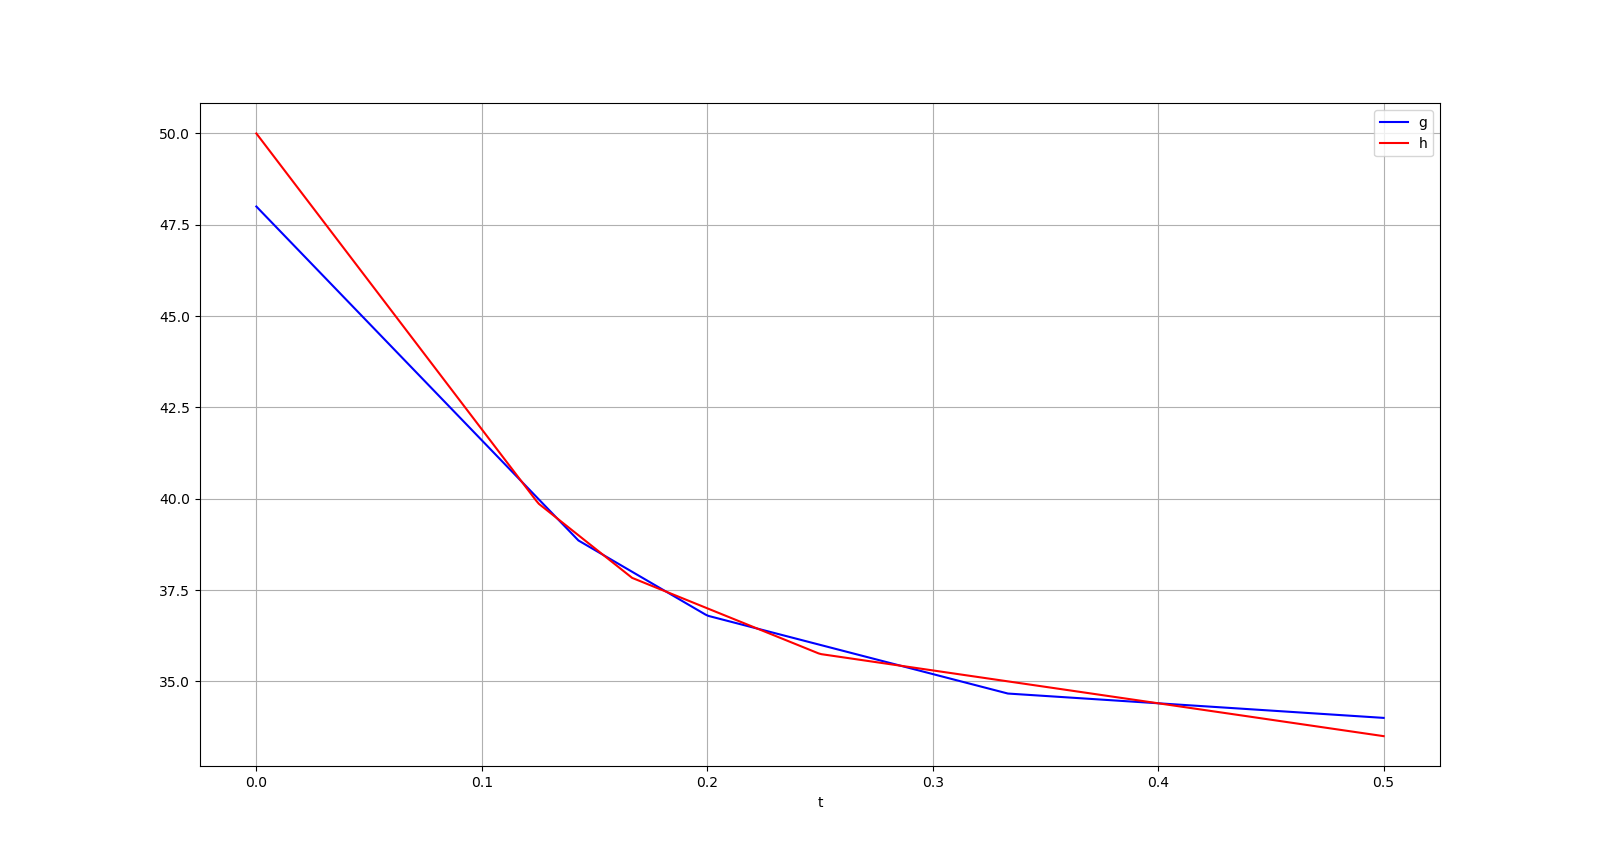
\includegraphics[scale=1, width=0.9\linewidth]{figures/chebyshev-eq-red.png}
		\caption{Example of the two functions constructed for the Chebyshev equation problem for the integer sequence \(1, 2, 3, 4\). The functions remain unchanged if any integer appears more than once.}
		\label{fig:chebyshev-eq-red}
	\end{figure}


	Define the function \(f_a(t) = C + 2a - a^2 t\), which corresponds to the terms inside the absolute values on both sides. The intuition is that \(f_a(t)\) is the tangent of \(C + 1/x\) at \(x = 1/a\). Note that \(f_a(1/a) > f_b(1/a)\) for all \(a \neq b \in \R_{> 0}\), because:
	\begin{alignat*}{3}
		& 0 &&< (b-a)^2 \\
		\iff & 0 &&> -\frac{1}{a}(b-a)^2 = 2b - \frac{b^2}{a} - a \\
		\iff & C + 2a - \frac{a^2}{a} &&> C + 2b - \frac{b^2}{a} \\
		\iff & f_a(1/a) &&> f_b(1/a).
	\end{alignat*}

	This means the functions \(g(t) = \max_{i=1,\dots, d} f_{2x_i}(t)\) and \(h(t) = \max_{i=1,\dots, d} f_{2x_i+1}(t)\) consist of exactly \(d'\) distinct line segments, where \(d'\) is the number of distinct elements in \(\{x_i\}\), as each distinct value contributes one segment. From \(t=0\) to \(t=1/2\), the segments are encountered in descending order of \(x_i\). The last segment is encountered at least after \(t=1/2\), since the smallest \(n = 2x_i\) is 2, so \(1/n \leq 1/2\).

	If all linear functions are positive on \([0, 1/2]\), then the absolute values can be removed, and \(g(t)\) and \(h(t)\) equal the left and right sides of \cref{eq:red-eq-chebyshev}, respectively. For \(C = \max_i 2x_i^2\), it can be verified that all terms are positive on \([0, 1/2]\).

	Now, consider the equation \(g(t) = h(t)\) on \([0, 1/2]\). At \(t = 1/(2x_i)\), we have \(g(t) > h(t)\), and at \(t = 1/(2x_i + 1)\), we have \(g(t) < h(t)\) for all \(i\). Let \(d'\) be the number of distinct \(x_i\). There are at least \(2d' - 1\) solutions because the sign of \(g(t)-h(t)\) alternates between these \(2d'\) points. However, there cannot be more than \(2d' - 1\) solutions because each of the \(d'\) segments in \(g\) can intersect the piecewise linear function \(h\) at most twice (since both are convex, and the first and last segments cannot both intersect \(h\) twice). Thus, the number of solutions in \([0, 1/2]\) is exactly \(2d' - 1\).

	To solve the distinctness problem, we construct \cref{eq:red-eq-chebyshev}, find the solutions in \([0, 1/2]\), and count them. The count is \(2d' - 1\), from which \(d'\) can be derived. Since element distinctness has an \(\Omega(d \log d)\) lower bound, the Chebyshev equation problem must also have this lower bound.
\end{proof}

\begin{lemma}
	The Manhattan equation problem (\cref{def:manhattan-problem}) has a lower bound of \(\Omega(d \log d)\).
\end{lemma}

\begin{proof}
	Given an instance of the integer element distinctness problem \(x_1, \dots, x_d \in \N_+\), we construct an instance of the Manhattan equation problem in \(2d\) dimensions:
	\begin{equation}\label{eq:red-eq-manhattan}
		1 + \sum_{i=1}^d |6x_i + 4 - 2t| = \sum_{i=1}^d \parenth{|3x_i + 1 - t| + |3x_i + 3 - t|}
	\end{equation}
	For examples, see \cref{fig:manhattan-eq-red-1,fig:manhattan-eq-red-2}. For a comparison of the component functions, see \cref{fig:manhattan-building-block}.

	\begin{figure}
	  \centering
	  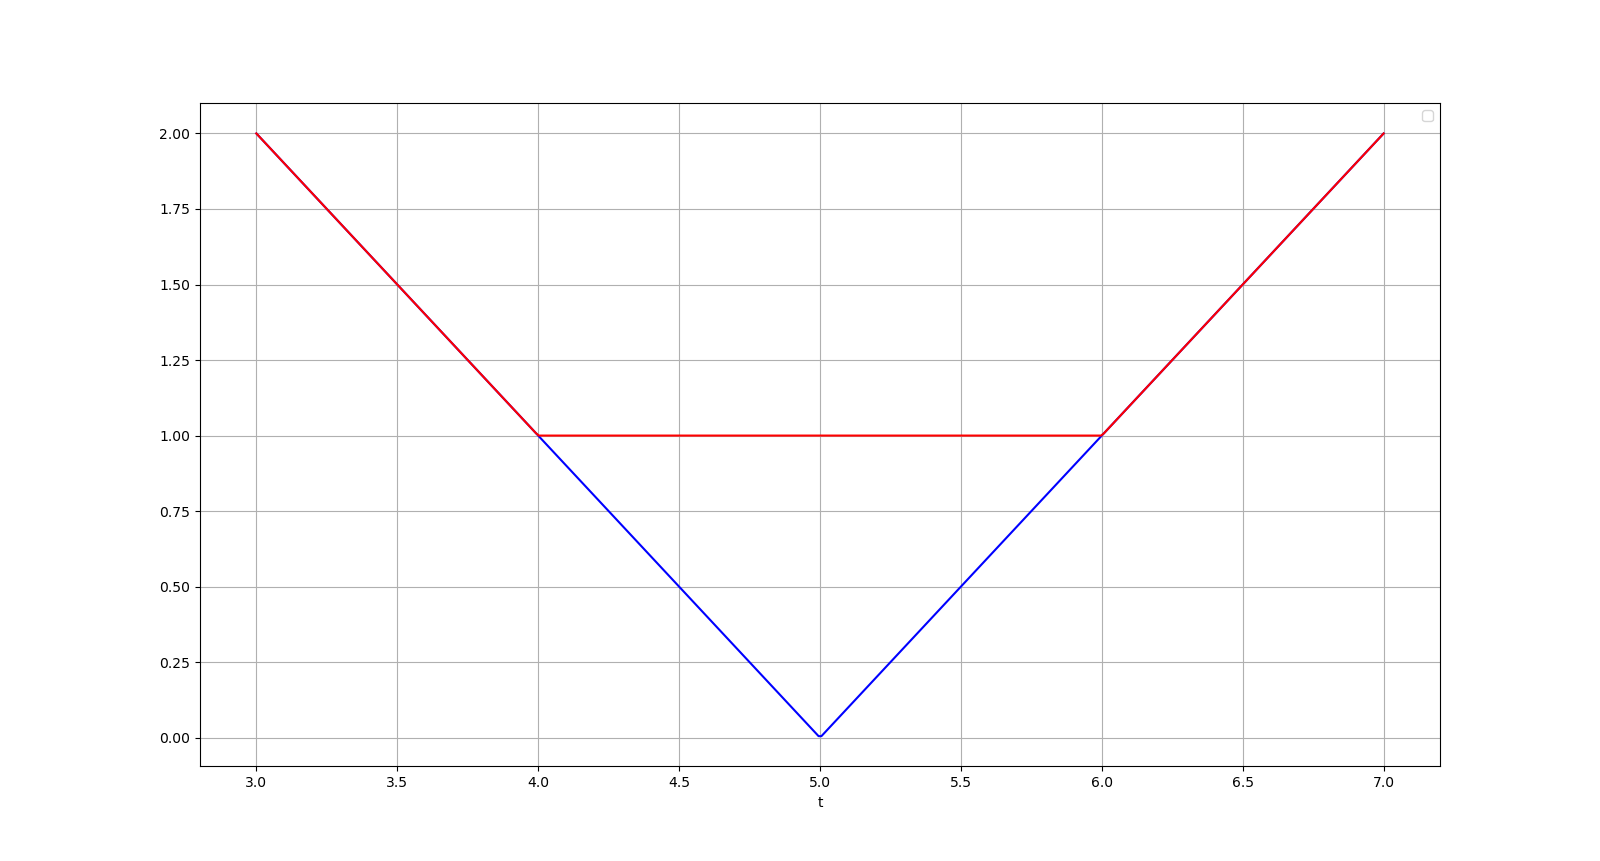
\includegraphics[scale=1, width=0.9\linewidth]{figures/manhattan-building-block.png}
	  \caption{Comparison of \(|6x_i + 4 - 2t|\) and \(|3x_i + 1 - t| + |3x_i + 3 - t|\) for \(x_i = 1\).}
	  \label{fig:manhattan-building-block}
	\end{figure}

	\begin{figure}
	  \centering
	  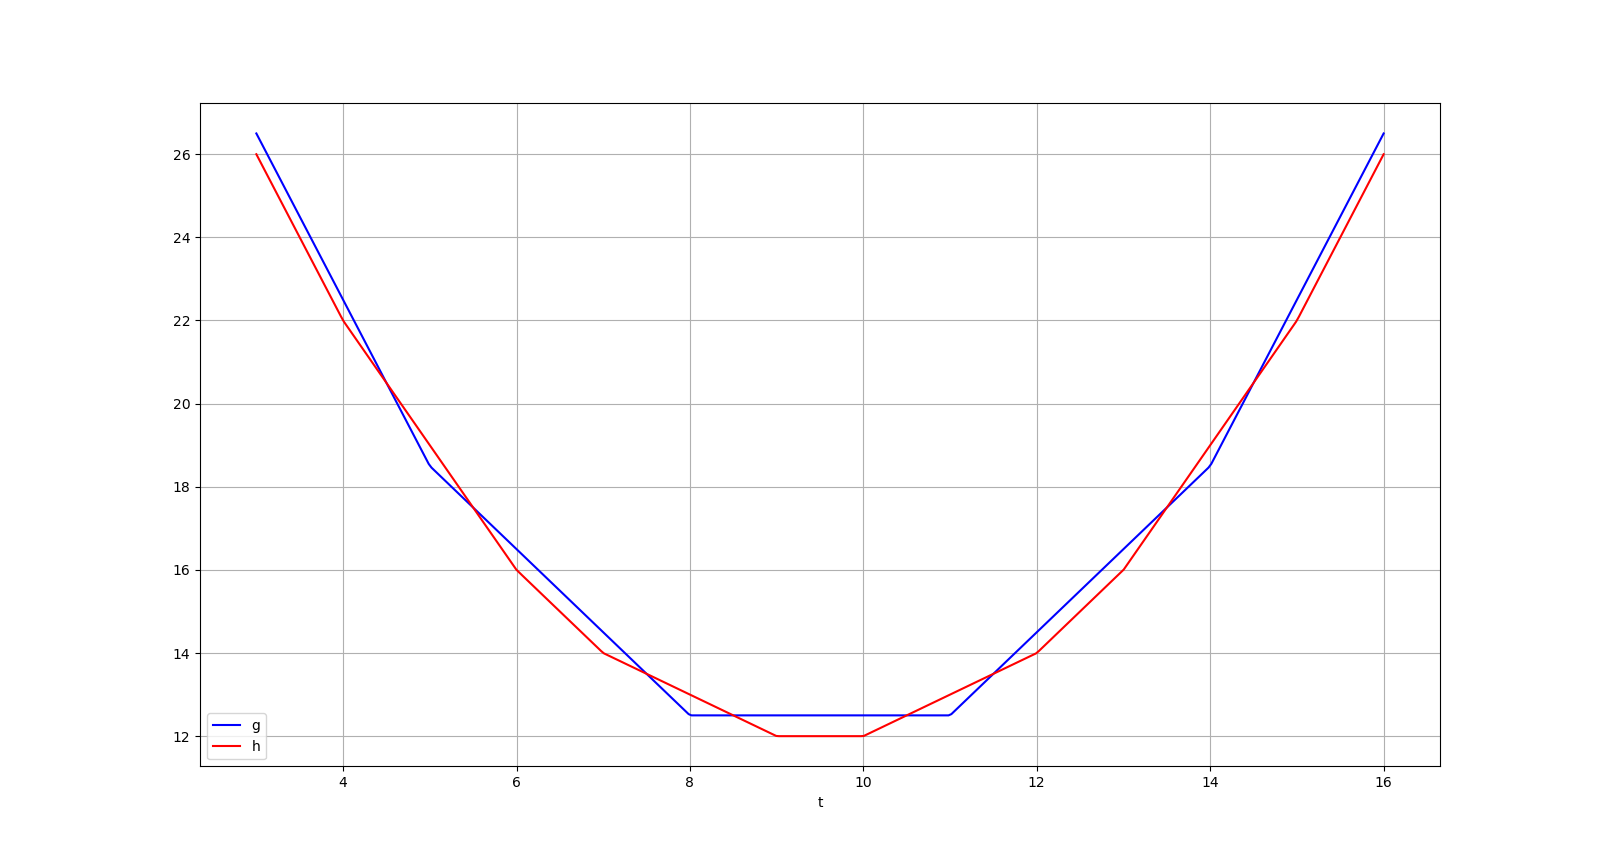
\includegraphics[scale=1, width=0.9\linewidth]{figures/manhattan-eq-red-1.png}
	  \caption{Instance for the numbers \(1,2,3,4\). There are 8 solutions, indicating 4 distinct values.}
	  \label{fig:manhattan-eq-red-1}
	\end{figure}

	\begin{figure}
	  \centering
	  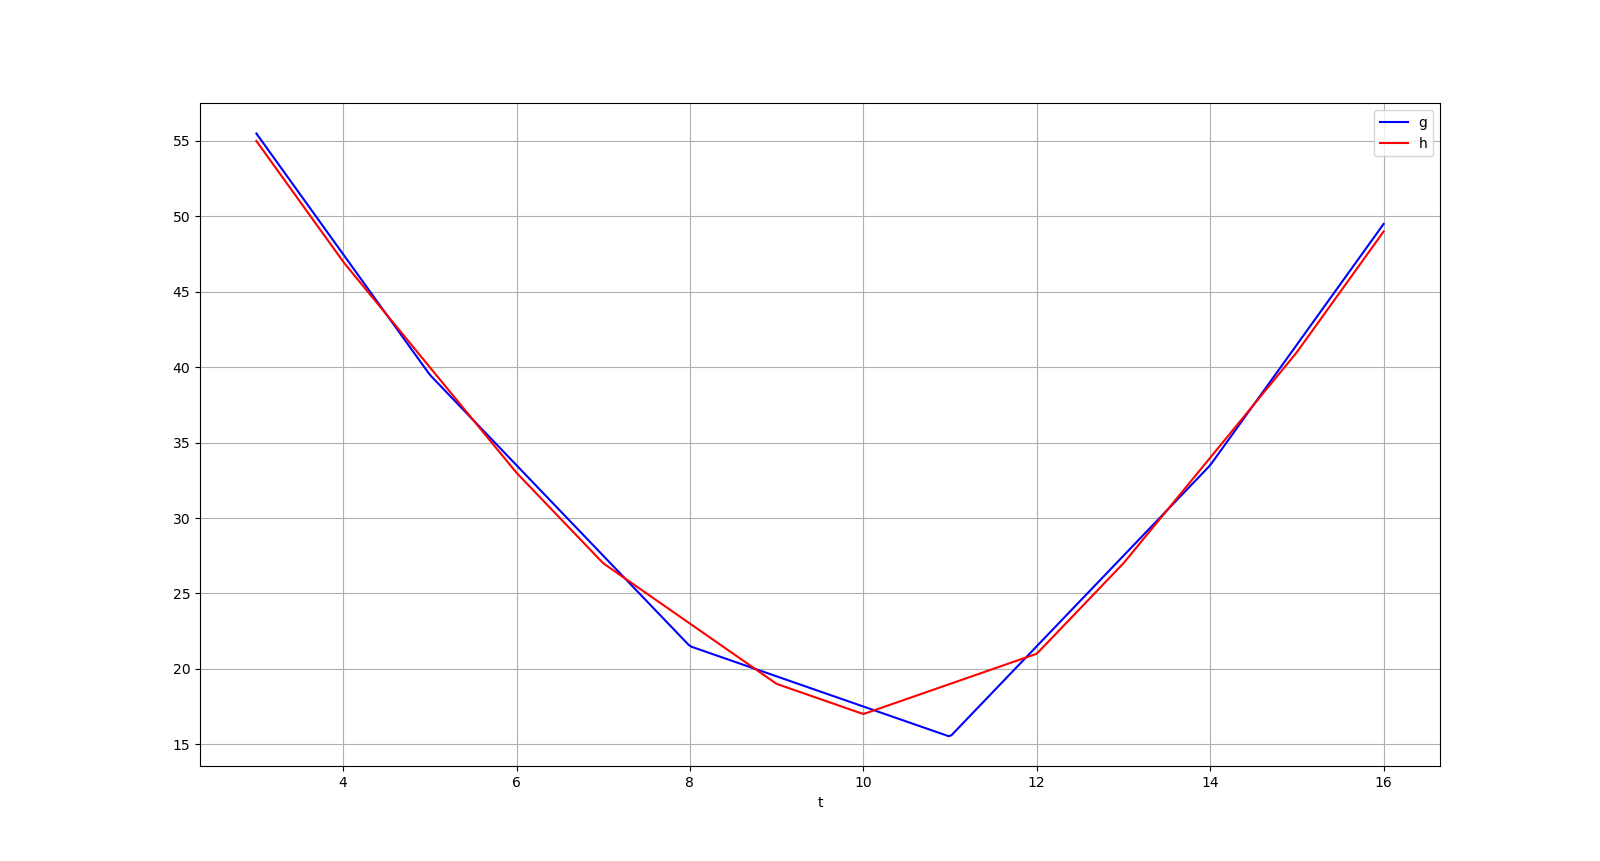
\includegraphics[scale=1, width=0.9\linewidth]{figures/manhattan-eq-red-2.png}
	  \caption{Instance for the numbers \(1,2,3,4,3,2,3,3\). Duplicates do not change the number of solutions but slightly shift their positions.}
	  \label{fig:manhattan-eq-red-2}
	\end{figure}

	Observe that for \(t \notin [3x_i + 1, 3x_i + 3]\), we have \(|6x_i + 4 - 2t| = |3x_i + 1 - t| + |3x_i + 3 - t|\). For \(t \in (3x_i + 1, 3x_i + 3)\), we have \(|6x_i + 4 - 2t| < |3x_i + 1 - t| + |3x_i + 3 - t|\). Furthermore, for any \(k \in \N_+\), the equation \(1 + k|6x_i + 4 - 2t| = k(|3x_i + 1 - t| + |3x_i + 3 - t|)\) has exactly two solutions in \([3x_i+1, 3x_i+3]\).

	Let \(g(t) = 1 + \sum_{i=1}^d |6x_i + 4 - 2t|\) and \(h(t) = \sum_{i=1}^d \parenth{|3x_i + 1 - t| + |3x_i + 3 - t|}\). For \(t \in [3x_i, 3x_i + 1]\) for any \(x_i\), we have \(g(t) = 1 + h(t)\). For \(t \in (3x_i+1, 3x_i + 3)\), the difference \(g(t) - h(t) = 1 + k|6x_i + 4 - 2t| - k(|3x_i + 1 - t| + |3x_i + 3 - t|)\), where \(k\) is the multiplicity of \(x_i\), has exactly two solutions in the interval. Thus, the total number of solutions is \(2d'\), where \(d'\) is the number of distinct values in \(\set{x_i}\). Therefore, solving the Manhattan equation problem allows us to determine \(d'\), and hence the lower bound applies.
\end{proof}
